\documentclass[cs4size,a4paper]{ctexart}   
\newcommand{\subsubsubsection}[1]{\paragraph{#1}\mbox{}\\}
\setcounter{secnumdepth}{4} % how many sectioning levels to assign numbers to
\setcounter{tocdepth}{4} % how many sectioning levels to show in ToC

%===数学符号公式===
\usepackage{amsmath}    					% AMS LaTeX宏包
\usepackage[style=1]{mdframed}
\usepackage{amsthm}
\usepackage{amssymb}
\usepackage{bm}                      	% 数学公式中的黑斜体
\usepackage{bbm}
\usepackage{amsfonts}
\usepackage{mathrsfs}                	% 英文花体字 体
\usepackage{bbding,manfnt}    			% 一些图标,如 \dbend
\usepackage{lettrine}                	% 首字下沉,命令\lettrine
\def\attention{\lettrine[lines=2,lraise=0,nindent=0em]{\large\textdbend\hspace{1mm}}{}}
\usepackage{longtable}
\usepackage{enumerate}
\usepackage[toc,page]{appendix}
\usepackage{geometry}         			% 页边距调整
\geometry{top=3.0cm,bottom=2.7cm,left=2.5cm,right=2.5cm}
\usepackage[colorinlistoftodos,prependcaption,textsize=small]{todonotes}
%===公式按章编号===
\numberwithin{equation}{section}
\numberwithin{table}{section}
\numberwithin{figure}{section}
%===基本格式预置===
\usepackage{fancyhdr}
\pagestyle{fancy}
\fancyhf{}  
\fancyhead[C]{\zihao{5}  \kaishu LaTeX软件使用指导}
\fancyfoot[C]{~\zihao{5} \thepage~}
\renewcommand{\headrulewidth}{0.75pt} 
\CTEXsetup[format={\centering\bfseries\zihao{-2}},name={第, 章}]{section}
\CTEXsetup[nameformat={\bfseries\zihao{3}}]{subsection}
\CTEXsetup[nameformat={\bfseries\zihao{4}}]{subsubsection}
%===图形支持宏包===
\usepackage{graphicx}        			% 嵌入png图像
\usepackage{subfigure}
\usepackage{float}
\graphicspath{{figure/}}
\usepackage{color,xcolor}     			% 支持彩色文本、底色、文本框等
\usepackage[colorlinks,linkcolor=blue,anchorcolor=blue,citecolor=blue]{hyperref}
% \usepackage{hyperref}
% \hypersetup{hidelinks,
% 	colorlinks=true,
% 	allcolors=black,
% 	pdfstartview=Fit,
% 	breaklinks=true}

%\usepackage{caption}
\usepackage[ruled,linesnumbered]{algorithm2e}
%\captionsetup{figurewithin=section}
%===源码和流程图===
\usepackage{listings,fontspec}         	% 粘贴源代码
\newfontfamily\monaco{Monaco}
\definecolor{mygreen}{rgb}{0,0.6,0}
\definecolor{mygray}{rgb}{0.5,0.5,0.5}
\definecolor{mymauve}{rgb}{0.58,0,0.82}
\lstset{ %
backgroundcolor=\color{white},   		% choose the background color
basicstyle=\footnotesize\monaco,       % size of fonts used for the code
columns=fullflexible,
breaklines=true,                 		% automatic line breaking only at whitespace
captionpos=b,                    		% sets the caption-position to bottom
tabsize=4,
commentstyle=\color{mygreen}\monaco,   % comment style
escapeinside={\%*}{*)},          		% if you want to add LaTeX within your code
keywordstyle=\color{blue}\monaco,      % keyword style
stringstyle=\color{mymauve}\monaco,    % string literal style
frame=single,
rulesepcolor=\color{red!20!green!20!blue!20},
% identifierstyle=\color{red},
language=python,
}
%===颜色===
\usepackage{color,xcolor}
\definecolor{dkgreen}{rgb}{0,0.6,0}
\definecolor{gray}{rgb}{0.5,0.5,0.5}
\definecolor{LetMeFlyGray}{RGB}{240,240,240}
\definecolor{mauve}{rgb}{0.58,0,0.82}
 \usepackage{xcolor}
 \lstset{
  %行号
   numbers=left,
   %背景框
   framexleftmargin=8mm,
   frame=none,
   %背景色
   %backgroundcolor=\color[rgb]{1,1,0.76},
   backgroundcolor=\color[RGB]{245,245,244},
   %样式
   keywordstyle=\bf\color{blue},
   identifierstyle=\bf,
   numberstyle=\color[RGB]{0,192,192},
   commentstyle=\it\color[RGB]{0,96,96},
   stringstyle=\rmfamily\slshape\color[RGB]{128,0,0},
   %显示空格
   showstringspaces=false,
   xleftmargin=2.5em
 }

%--------------------
\hypersetup{hidelinks}
\usepackage{booktabs}  
\usepackage{shorttoc}
\usepackage{tabu,tikz}
\usepackage{float}
\usepackage{multirow}

\tabcolsep=1ex
\tabulinesep=\tabcolsep
\newlength\tikzboxwidth
\newlength\tikzboxheight
\newcommand\tikzbox[1]{%
        \settowidth\tikzboxwidth{#1}%
        \settoheight\tikzboxheight{#1}%
        \begin{tikzpicture}
        \path[use as bounding box]
                (-0.5\tikzboxwidth,-0.5\tikzboxheight)rectangle
                (0.5\tikzboxwidth,0.5\tikzboxheight);
        \node[inner sep=\tabcolsep+0.5\arrayrulewidth,line width=0.5mm,draw=black]
                at(0,0){#1};
        \end{tikzpicture}%
        }
\makeatletter
\def\hlinew#1{%
  \noalign{\ifnum0=`}\fi\hrule \@height #1 \futurelet
   \reserved@a\@xhline}
   

\usepackage{ifthen}
\newcommand{\HRule}{\rule{\linewidth}{0.5mm}}
\newcommand{\tabincell}[2]{\begin{tabular}{@{}#1@{}}#2\end{tabular}}%
%===使得公式随章节自动编号===
\makeatletter
\@addtoreset{equation}{section}
\makeatother
\renewcommand{\theequation}{\arabic{section}.\arabic{equation}}
%-------------------------
\usepackage{pythonhighlight}
\usepackage{tikz}                    
\usepackage{tikz-3dplot}
% \usepackage{hyperref}
\usetikzlibrary{shapes,arrows,positioning}
%===正文开始===
\begin{document}
%===定理类环境定义===
\newtheorem{example}{例}              	% 整体编号
\newtheorem{algorithem}{算法}	
\newtheorem{theorem}{定理}            	% 按section编号
\newtheorem{definition}{定义}
\newtheorem{axiom}{公理}
\newtheorem{property}{性质}
\newtheorem{proposition}{命题}
\newtheorem{lemma}{引理}
\newtheorem{corollary}{推论}
\newtheorem{remark}{注解}
\newtheorem{condition}{条件}
\newtheorem{conclusion}{结论}
\newtheorem{assumption}{假设}
%===重定义===
\renewcommand{\contentsname}{目录}     
\renewcommand{\abstractname}{摘要} 
\renewcommand{\refname}{参考文献}     
\renewcommand{\indexname}{索引}
\renewcommand{\figurename}{图}
\renewcommand{\tablename}{表}
\renewcommand{\appendixname}{附录}
\renewcommand{\proofname}{证明}
%\renewcommand{\algorithm}{算法} 
\renewcommand\emph[1]{\textcolor{red}{\textbf{#1}}}
%===封皮和前言===
\begin{titlepage}
\begin{center}
% Upper part of the page

\includegraphics[width=0.25\textwidth]{logo}\\[1cm]    
%\textsf{\LARGE\bfseries Natural selection, Survival of the fittest.}\\[1.0cm]
\textsf{\Large\bfseries Beijing University of Chemical Technology}\\[1.0cm]
\textsc{\Large Dynamic Time Warping}\\[0.5cm]
% Title
\HRule \\[0.8cm]
{\huge \bfseries 生产实习报告}\\[0.4cm]
\HRule \\[0.7cm]
% Author
\textsf{\bfseries 计科1906 李腾飞}
\tableofcontents 
\vfill
% Bottom of the page
{创建日期:2022年8月28日}\\
{更新日期:\today}
\end{center}
\end{titlepage}
\pagestyle{plain}
\pagenumbering{Roman}
\thispagestyle{empty}
%===正文===
\pagestyle{fancy}
\pagenumbering{arabic}



\section{论文概述}

基于经验模式分解和希尔伯特-黄变换的瞬时三维脑电信号分析应用于麻醉深度。

可执行文件下载:\url{https://letmefly.xyz/Links/Redirect/id.html?21} (必须和\href{https://github.com/LetMeFly666/Instantaneous3D_EEG_SignalAnalysis/releases/download/v0.1.0/case7.txt}{case7.txt}放在相同目录下使用)

\subsection{论文中的名词中英文对照}

\begin{table}[H]
\caption{ 英文名词缩写-中文名词对照表}
\centering
\begin{tabular}{r|l}
\toprule
英文缩写 & 中文\\
\midrule[2pt]
DoA & Depth of anaesthesia(麻醉深度)\\
EEG & electroencephalography(脑电图学)\\
EMD & empirical mode decomposition(经验模态分解)\\
HHT & Hilbert–Huang transform(希尔伯特-黄变换)\\
HT & Hilbert transform(希尔伯特变换)\\
IMF & intrinsic mode functions(固有模态函数)\\
SampEn & sample entropy(样本熵)\\
BIS & bispectral index(脑电双频指数)\\
ECG & electrocardiography(心电描记术)\\
FFT & Fast Fourier Transform(快速傅里叶变换)\\
AUC ratio of \\$\alpha$ + $\beta$ waves & area ratio of $\alpha$ + $\beta$ waves (8–32 Hz) under\\ &FFT curve(快速傅立叶变换曲线下$\alpha$+$\beta$波(8-32赫兹)的面积比)\\
EMG & electromyography(肌电图描记法)\\
EOG & electrooculography(眼动电图描记法)\\
ESUs & electrosurgical units(电外科装置)\\
IFFT & Inverse fast Fourier transform(快速傅里叶逆变换)\\
ApEn & approximate entropy(近似熵)\\
\bottomrule
\end{tabular}
\end{table}

\subsection{预备知识}

\subsubsection{时域和频域}

时域是客观世界中唯一实际存在域;频域是一个数学构造,也被一些学者称为上帝视角。

\subsubsection{时域}

以时间轴为坐标表示动态信号的关系

\subsubsection{频域}

正弦波是频域中唯一存在的波形

\subsubsection{转换}

动态信号从时间域变换到频率域主要通过傅立叶级数和傅立叶变换实现。周期信号靠傅立叶级数,非周期信号靠傅立叶变换。时域越宽,频域越短。

\subsection{论文摘要}

麻醉的程度(DoA)是评估全身麻醉剂对患者中枢神经系统抑制程度的重要指标。通过监测病人脑电信号(electroencephalography(EEG))来判断病人是否处于全麻状态有助于调节DoA并减轻手术的风险。

\subsection{介绍}

EMD可以从原始EEG信号中滤除噪音相关的频率,并可以结合挑选出来的固有模态函数得到滤波后的EEG信号。之后在滤波后的EEG信号的基础上用HHT得到瞬时频率和瞬时振幅。

之后就可以用“瞬时频率、瞬时振幅和EEG信号中的时间元素”重组并构建 可以实时显示脑电信号振幅和频率的 实时3D表示图。

\section{论文复现方法简述}

\begin{figure}  
    \scriptsize  
    \tikzstyle{format}=[rectangle,draw,thin,fill=white]  
    %定义语句块的颜色,形状和边
    \tikzstyle{test}=[diamond,aspect=2,draw,thin]  
    %定义条件块的形状,颜色
    \tikzstyle{point}=[coordinate,on grid,]  
    %像素点,用于连接转移线
    \begin{tikzpicture}%[node distance=10mm,auto,>=latex',thin,start chain=going below,every join/.style={norm},] 
    %start chain=going below指明了流程图的默认方向,node distance=8mm则指明了默认的node距离。这些可以在定义node的时候更改,比如说 
    %\node[point,right of=n3,node distance=10mm] (p0){};  
    %这里声明了node p0,它在node n3 的右边,距离是10mm。
    \node[format,anchor=center] (start){Raw EEG signal};
    \node[format,below of=start,node distance=11mm] (define){Step 1.\\Decompose into IMF};
    \node[format,below of=define,node distance=11mm] (PCFinit){Step 2.\\Convert to frequency domain};
    \node[format,below of=PCFinit,node distance=11mm] (DS18init){Step 3.\\Cut off the noise};
    \node[format,below of=DS18init,node distance=11mm] (LCDinit){Step 4.\\Reverse into time domain};
    \node[format,below of=LCDinit,node distance=11mm] (processtime){Step 5.\\Construct filtered EEG};
    \node[format,below of=processtime,node distance=11mm] (keyinit){Step 6.\\Obtain instantaneous frequency};
    \node[format,below of=keyinit,node distance=11mm] (lastStep){Step 7.\\Build the 3D representation};
    %\node[format] (n0) at(4,4){A}; 直接指定位置 
    %定义完node之后进行连线,
    %\draw[->] (n0.south) -- (n1); 带箭头实线
    %\draw[-] (n0.south) -- (n1); 不带箭头实线
    %\draw[<->] (n0.south) -- (n1.north);   双箭头
    %\draw[<-,dashed] (n1.south) -- (n2.north); 带箭头虚线 
    %\draw[<-] (n0.south) to node{Yes} (n1.north);  带字,字在箭头方向右边
    %\draw[->] (n1.north) to node{Yes} (n0.south);  带字,字在箭头方向左边
    %\draw[->] (n1.north) to[out=60,in=300] node{Yes} (n0.south);  曲线
    %\draw[->,draw=red](n2)--(n1);  带颜色的线
    \draw[->] (start)--(define);
    \draw[->] (define)--(PCFinit);
    \draw[->](PCFinit)--(DS18init);
    \draw[->](DS18init)--(LCDinit);
    \draw[->](LCDinit)--(processtime);
    \draw[->](processtime)--(keyinit);
    \draw[->](keyinit)--(lastStep);
    \end{tikzpicture}  
\caption{ 方法流程图}
\end{figure}

% 居中不了呜呜

\subsection{step1 将原有EEG信号分解为数个IMF}

$$x(t)=\sum_{i=1}^{n} c_{i}(t)+r_{n}(t)$$

$x(t)$是时域下的原始信号,$c_i(t)$是第$i$个IMF(固有模态函数),$r_n(t)$是残余信号。

\subsection{step2 将IMF转换到频域}

使用FFT将IMF从时域转换到频域。

\subsection{step3 去除每个IMF中的噪声}

人脑产生的脑电信号的正常频率在0.5赫兹Hz到32Hz之间,它们分别包含从低频到高频的$\delta$,$\theta$,$\alpha$波和$\beta$波。

\subsection{step4 将IMF转回到时域}

使用快速傅立叶逆变换IFFT

\subsection{step5 构造滤波后的脑电信号的IMF}

IFFT带来的边缘效应会使前5秒和后5秒的振幅异常地高,因此去掉前5秒和后5秒。

丢掉过小的IMF。

\subsection{step6 通过HHT获得实时频率}

$\delta$ (0.5–4 Hz), $\theta$ (4–8 Hz), $\alpha$ (8–16 Hz), $\beta$ (16–32 Hz)

Other: Noise

\subsection{step7 构建三维表示}

x轴:频率,y轴:时间,z轴:振幅

\section{具体实现}

\begin{enumerate}
\item \colorbox{LetMeFlyGray}{Codes/main.py}:主程序,主要负责调用
\item \colorbox{LetMeFlyGray}{Codes/BaseClass.py}:数据类,包括数据、起始截止时间、采样频率等
\item \colorbox{LetMeFlyGray}{Codes/BaseFunction.py}:一些基本的函数功能
\item \colorbox{LetMeFlyGray}{Codes/LetEMD.py}:实现了EEG的EMD分解
\item \colorbox{LetMeFlyGray}{Codes/Visualize.py}:将数据可视化
\item \colorbox{LetMeFlyGray}{Codes/Txt2numpy.py}:读取数据
\item \colorbox{LetMeFlyGray}{Codes/ShowOriginalEEGdata.py}:显示原始EEG
\item \colorbox{LetMeFlyGray}{Codes/Data2IMFs.py}:将数据分成很多IMF、将IMF转换到频域
\item \colorbox{LetMeFlyGray}{Codes/IMFs2FrequencyDomain.py}:将IMF转换到频域
\item \colorbox{LetMeFlyGray}{Codes/CutoffNoice.py}:将信号中不符合频率范围的部分删除
\item \colorbox{LetMeFlyGray}{Codes/IMF2TimeDomain.py}:将IMF转回时域
\item \colorbox{LetMeFlyGray}{Codes/ConstructEEG.py}:将IMF构建回EEG(并去除前10s的信号)
\item \colorbox{LetMeFlyGray}{Codes/HHT.py}:通过HHT获得实时频率
\item \colorbox{LetMeFlyGray}{Codes/ShowRealtime3D.py}:显示为实时三维图
\end{enumerate}

\subsection{主程序main.py}

\colorbox{LetMeFlyGray}{main.py}是总函数,主要负责函数调用。

主要包括“导入所需库”、“取消QT警告”和“调用其他写好的函数”

\subsubsection{导入所需库}

这一小节没有太多需要讲述的。在这一小节中,所导入的\textbf{全部}是我自己实现的功能,每个库实现一个小功能,具体实现的时候很多地方使用到了现成库。

\begin{lstlisting}[language={python},
    numbers=left,
    numberstyle=\tiny\monaco,
    basicstyle=\footnotesize\monaco]
from Txt2numpy import txt2numpy
from ShowOriginalEEGdata import showOriginalEEGdata
from Data2IMFs import data2IMFs
from IMFs2FrequencyDomain import IMFs2FrequencyDomain
from CutoffNoise import cutoffNoise
from IMF2TimeDomain import IMF2TimeDomain
from ConstructEEG import ConstructEEG
from HHT import HHT
from ShowRealtime3D import showRealtime3D
\end{lstlisting}

\subsubsection{取消QT警告}

因为我电脑上安装了QT(并将QT安装配置过程写成了笔记),因此在使用\colorbox{LetMeFlyGray}{matplotlib}画图的时候,控制台就会输出QT警告。

因此,这里参考\url{https://www.likecs.com/ask-924744.html},通过临时改变一些环境变量,达到了消除警告的目的。

\begin{lstlisting}[language={python},
numbers=left,
numberstyle=\tiny\monaco,
basicstyle=\footnotesize\monaco]
import os
# 取消QT警告
os.environ["QT_DEVICE_PIXEL_RATIO"] = "0"
os.environ["QT_AUTO_SCREEN_SCALE_FACTOR"] = "1"
os.environ["QT_SCREEN_SCALE_FACTORS"] = "1"
os.environ["QT_SCALE_FACTOR"] = "1"
\end{lstlisting}

\subsubsection{调用其他写好的函数}

主函数的最后一个任务就是调用其他写好的函数,包括:

\begin{lstlisting}[language={python},
numbers=left,
numberstyle=\tiny\monaco,
basicstyle=\footnotesize\monaco]
EEG = txt2numpy()  # 从文本文件读入数据
showOriginalEEGdata(EEG)  # 显示原本EEG文件
IMFs = data2IMFs(EEG)  # step1.将EEG数据转换为IMF
IMFs = IMFs2FrequencyDomain(IMFs=IMFs)  # step2.将IMF转换到频域
IMFs = cutoffNoise(IMFs=IMFs)  # step3.去除每个IMF中的噪声
IMFs = IMF2TimeDomain(IMFs=IMFs)  # step4.转回到时域
EEG = ConstructEEG(IMFs=IMFs)  # step5.选取有效范围的IMF并构建EEG
instantaneousFrequency = HHT(EEG)  # step6.通过HHT获得实时频率
showRealtime3D(EEG, instantaneousFrequency)  # step7.显示为实时三维图
\end{lstlisting}

\subsection{基本数据类 BaseClass.py}

\colorbox{LetMeFlyGray}{BaseClass.py}主要实现了基本的数据类,包括数据、数据的采样频率、起始采样时间等。

\subsubsection{所支持数据类型}

这个函数中仅有一个实现好的类\colorbox{LetMeFlyGray}{Data},它支持一维数据和二维数据。

\begin{table}[H]
\caption{Data类所支持的数据类型}
\centering
\begin{tabular}{l|l}
\toprule
数据类型 & 例\\
\midrule[2pt]
一维数据:[1, 2, 1, 2, 3, ...]  & Example: data.shape = (500, )\\
二维数据:[[1, 2, 1, ..], [2, 6, 3, ..], ..]  &Example: data.shape = (5, 500) \\
\bottomrule
\end{tabular}
\end{table}

\subsubsection{成员}

成员包括变量和方法。

\subsubsubsection{变量}

\begin{table}[H]
\caption{Data成员变量及其意义}
\centering
\begin{tabular}{l|l}
\toprule
成员变量 & 解释说明\\
\midrule[2pt]
data: np.ndarray & 主要数据\\
dataLength & 数据的长度。这里时指单条数据共采样了多少次\\
startTime & 数据的开始采样时间 \\
endTime & 数据的结束采样时间\\ & [startTime, endTime)\\
FPS & 每秒采样多少次\\
\bottomrule
\end{tabular}
\end{table}

\subsubsubsection{方法}

\begin{table}[H]
\caption{Data成员方法及其意义}
\centering
\begin{tabular}{l|l}
\toprule
成员方法 & 解释说明\\
\midrule[2pt]
getData() -> np.ndarray &  获取采样数据\\
getDataLength(data: np.ndarray) -> int &  获取数据的长度(采样次数)\\
getStartTime() -> float & 获取数据的开始采样时间\\
getEndTime() -> float & 获取数据的结束采样时间\\
getFPS() -> int & 获取数据的采样频率\\
getTimeRangeArray() -> np.ndarray &  获取时间的数组(数组中为所有的采样时刻)\\
setSubDataByPoints(frontSkippedPoints: int,\\ backSkippedPoints: int) -> None &  设置数据为子数据(通过采样点来设置)\\
setSubDataByTime(frontSkippedTime: float,\\ backSkippedTime: float) -> None &  设置数据为子数据(通过时间来设置)\\
\bottomrule
\end{tabular}
\end{table}

\subsubsection{构造函数的参数}

\begin{enumerate}
\item startTime
\item endTime
\item FPS
\end{enumerate}

具体含义可参考“成员变量”中的解释。

\subsection{可视化 Visualize.py}

\colorbox{LetMeFlyGray}{Visualize.py}主要实现数据的可视化。

此模块一共实现了三种可视化功能:“可视化EEG(一组数据)”、“可视化IMF(多组数据)”和“结果3D可视化”。

可视化部分主要使用了3个库:

\begin{enumerate}
\item 一个是\colorbox{LetMeFlyGray}{numpy}库,用于3D显示中对数据的处理。
\item 一个是\colorbox{LetMeFlyGray}{matplotlib}库,用于数据的可视化和图形的显示。
\item 一个是我构造的\colorbox{LetMeFlyGray}{BaseClass}库中的\colorbox{LetMeFlyGray}{Data}类,因为整个程序中,数据都是在\colorbox{LetMeFlyGray}{Data}类中存储的。
\end{enumerate}

\subsubsection{显示EEG图像}

EEG数据有一个时间轴,剩下的就是数据了。因此,可以使用matplotlib很方便地显示。

\begin{lstlisting}[language={python},
numbers=left,
numberstyle=\tiny\monaco,
basicstyle=\footnotesize\monaco]
def showEEG(EEG: Data, title="EEG") -> None:
    ax = plt.subplot()
    ax.set_title(title)
    ax.plot(EEG.getTimeRangeArray(), EEG.data)
    plt.show()
\end{lstlisting}

程序接受两个参数,一个是自定义Data类的待显示数据,一个是显示的图表的标题。

\subsubsection{显示IMF图像}

一般IMF不只一个,因此这个函数就是要将每一个IMF分别显示

\begin{lstlisting}[language={python},
numbers=left,
numberstyle=\tiny\monaco,
basicstyle=\footnotesize\monaco]
def showIMFs(IMFs: Data, title="IMFs") -> None:
    fig, axes = plt.subplots(IMFs.data.shape[0], 1)
    if IMFs.data.shape[0] == 1:
        axes = list(axes)
    axes[0].set_title(title)
    for num, IMF in enumerate(IMFs.data):
        ax = axes[num]        
        ax.plot(IMFs.getTimeRangeArray(), IMF)
        ax.set_ylabel("IMF " + str(num + 1))
    plt.show()
\end{lstlisting}

程序接受两个参数,一个是自定义Data类的待显示数据,一个是显示的图表的标题。

\subsubsection{显示3D图}

3D图将显示最终信号的时间轴、频率、相位,由此可以较为明显地观察到算法实现的效果。

\begin{lstlisting}[language={python},
numbers=left,
numberstyle=\tiny\monaco,
basicstyle=\footnotesize\monaco]
def show3d(F: Data, A: Data, ColorfulAndResize=False):
    x_F = F
    y_time = A.getTimeRangeArray()
    z_A = A

    fig = plt.figure()
    ax = fig.add_subplot(111, projection='3d')

    if ColorfulAndResize:
        colors = []
        for f in x_F.data:
            if f < 0.5:
                colors.append("red")
            elif f < 4:
                colors.append("blue")
            elif f < 8:
                colors.append("yellow")
            elif f < 16:
                colors.append("green")
            elif f < 32:
                colors.append("pink")
            else:
                colors.append("red")
        im = ax.scatter(np.abs(x_F.data), y_time, np.abs(z_A.data), c=colors, s=1)  # s: 点的大小
        ax.set_zlim(0, 1000)
        ax.set_title("Colorful & Resize")
    else:
        im = ax.scatter(np.abs(x_F.data), y_time, np.abs(z_A.data), s=1)  # s: 点的大小
        

    ax.set_xlabel("x_F")
    ax.set_ylabel("y_time")
    ax.set_zlabel("z_A")
    plt.show()

\end{lstlisting}

程序接受三个参数,一个是自定义Data类的频率数据,一个是自定义Data类的相位,最后一个参数决定是否像论文中的格式那样显示图表(以便和论文中的结果进行对照)。


其中,不同频率的数据显示不同的颜色的方法学习自\url{https://www.jb51.net/article/258747.htm},绘制三维散点图的方法学习自\url{https://blog.csdn.net/weixin\_46287157/article/details/124784731}



\subsection{数据读取 Txt2numpy.py}

\colorbox{LetMeFlyGray}{Txt2numpy.py}主要实现数据的读取。

\subsubsection{数据来源}

这里不得不提一提数据的来源。论文中为注明数据的来源,我尝试了很多类型的数据都和论文中的数据差别较大。

我尝试向论文中的通讯地址发送了一封邮件,请求作者分享一份数据给我,但是邮件始终未得到回复。

最终,我在承勇老师提供的一个链接里下载到了一个合适的数据。

下载地址:\url{https://figshare.com/articles/dataset/EEG_and_BIS_raw_data/5589841/1
}

case7.txt是case7.mat读入matlab后,将EEG取第1到4000个元素,并保存到文件后得到的。

Matlab保存数据到文件的代码为:

\begin{lstlisting}[language={matlab},
numbers=left,
numberstyle=\tiny\monaco,
basicstyle=\footnotesize\monaco]
dlmwrite('case7.txt', EEG(1: 4000), 'delimiter', ' ')
\end{lstlisting}

此方法学习自CSDN:\url{https://blog.csdn.net/whb12345678feng/article/details/103108114}

\subsection{读取数据}

OK,既然我们得到了数据,那么就可以开始愉快地将数据读入Python了。

\begin{lstlisting}[language={python},
        numbers=left,
        numberstyle=\tiny\monaco,
        basicstyle=\footnotesize\monaco]
import numpy as np
from BaseClass import Data
def txt2numpy(file="../Data/case7.txt") -> Data:
        arr = np.loadtxt(file)
        return Data(arr, 0, 100)  # 开始时间、采样频率
\end{lstlisting}

\subsubsection{说明}

虽然代码不是很长,但是把这个功能专门抽象出一个\colorbox{LetMeFlyGray}{.py}文件出来,是为了方便日后程序的拓展与完善。如:支持多种数据格式的读取、支持频率的设定等。

\subsection{显示原有EEG信号 ShowOriginalEEGdata.py}

\colorbox{LetMeFlyGray}{ShowOriginalEEGdata.py}可视化显示原始EEG信号(处理前)

\subsubsection{简介}

前面我们已经实现了EEG信号的展示函数,因此这里就会非常方便,只需要调用一下前面实现的函数即可。

如果想要手动实现也很简单:

\begin{lstlisting}[language={python},
numbers=left,
numberstyle=\tiny\monaco,
basicstyle=\footnotesize\monaco]
from matplotlib import pyplot as plt
from BaseClass import Data

def showOriginalEEGdata(EEG: Data) -> None:
    ax = plt.subplot()
    ax.set_title('Original EEG')
    ax.plot(EEG.getTimeRangeArray(), EEG.getData())
    plt.show()
\end{lstlisting}

\subsubsection{效果展示}

\begin{figure}[H]
\small
\centering
% 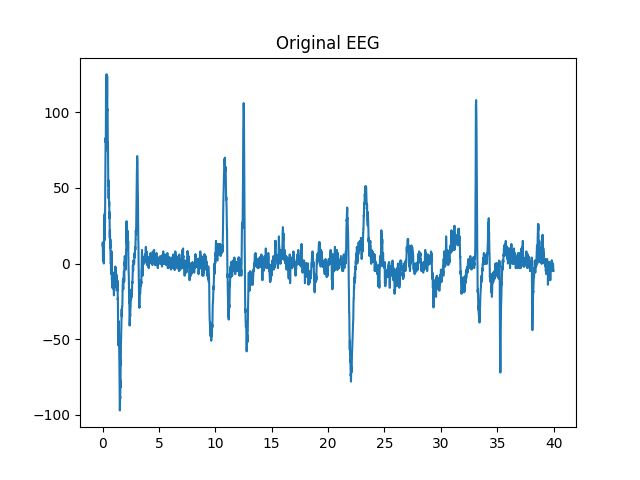
\includegraphics[width=\textwidth]{OriginalEEG.png}
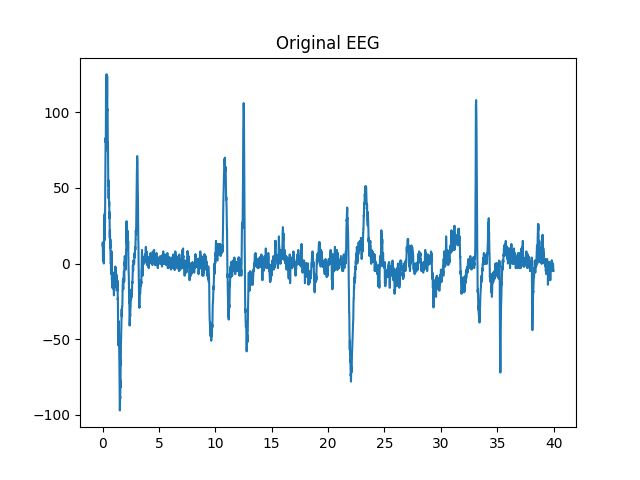
\includegraphics{OriginalEEG.png}
\caption{OriginalEEG} \label{fig:OriginalEEG}
\end{figure}

\subsection{分解EEG为数个IMF Data2IMFs.py}

\colorbox{LetMeFlyGray}{Data2IMFs.py}实现了一些EEG信号处理领域所需的功能

\subsubsection{简介}

在这里我花费了较多的精力,也写了较多的代码,我将EMD的实现抽象成了一个.py文件,后面会讲具体实现原理。

这个文件的目的是调用另外一个文件\colorbox{LetMeFlyGray}{LetEMD.py}将原始EEG信号分解为数个IMF和“剩余部分”

同时,这个文件又手动实现了一遍数据的可视化展示,因为我实现的可视化展示类中,不支持显示“Residue”这个标题

\begin{lstlisting}[language={python},
numbers=left,
numberstyle=\tiny\monaco,
basicstyle=\footnotesize\monaco]
from LetEMD import EMD
from matplotlib import pyplot as plt
from BaseClass import Data


def data2IMFs(data: Data):
    emd = EMD()
    IMFs, residue = emd.emd(data.getData())

    fig, axes = plt.subplots(IMFs.shape[0] + 1, 1)
    if IMFs.shape[0] == 1:
        axes = list(axes)
    axes[0].set_title("The IMFs")
    for num, IMF in enumerate(IMFs):
        axes[num].plot(data.getTimeRangeArray(), IMF)
        axes[num].set_ylabel("IMF " + str(num + 1))
    axes[IMFs.shape[0]].plot(data.getTimeRangeArray(), residue)
    axes[IMFs.shape[0]].set_ylabel("Residue")
    
    plt.show()

    return Data(IMFs, data.getStartTime(), data.getFPS())
\end{lstlisting}

\subsubsection{实现效果}

\begin{figure}[H]
\small
\centering
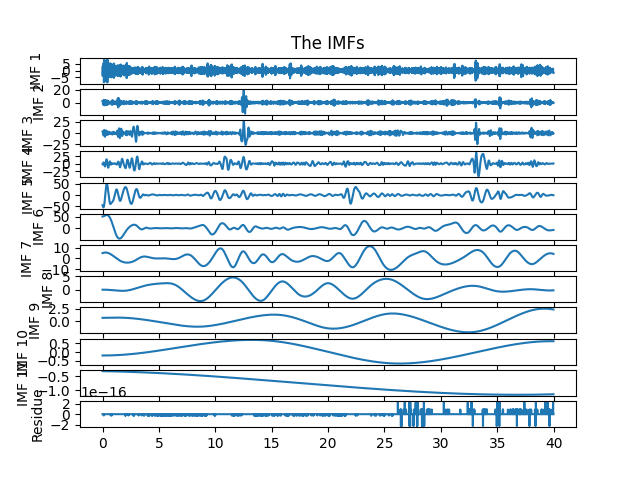
\includegraphics{IMFs.png}
\caption{IMFs} \label{fig:IMFs}
\end{figure}

\subsection{将IMF转到频域 IMFs2FrequencyDomain.py}

\colorbox{LetMeFlyGray}{IMFs2FrequencyDomain.py}使用快速傅里叶变换将IMF由时域转换到了频域

\subsubsection{简介}

手动实现EMD花费了我很多的时间,在时间不是很充裕的前提下,我调用了\colorbox{LetMeFlyGray}{scipy.fftpack}中实现好的FFT函数完成了快速傅里叶变换,而没有再手动实现一遍。

\begin{lstlisting}[language={python},
numbers=left,
numberstyle=\tiny\monaco,
basicstyle=\footnotesize\monaco]
from scipy.fftpack import fft
import numpy as np
from Visualize import showIMFs
from BaseClass import Data

def IMFs2FrequencyDomain(IMFs: Data):
    for num, IMF in enumerate(IMFs.getData()):
        frequency = fft(IMF)
        magnitude = np.abs(frequency)
        phase = np.angle(frequency)
        IMFs.data[num] = magnitude

    showIMFs(IMFs, "Change IMFs into frequency domain")    
    return IMFs
\end{lstlisting}

\subsubsection{实现效果}

\begin{figure}[H]
\small
\centering
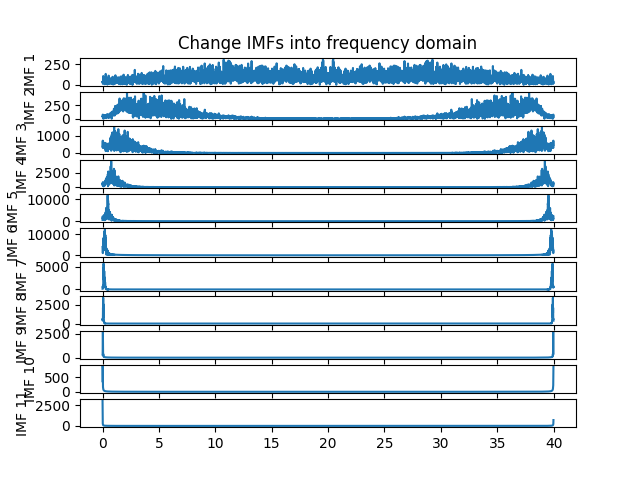
\includegraphics{IMF2FrequencyDomain.png}
\caption{IMF2FrequencyDomain} \label{fig:IMF2FrequencyDomain}
\end{figure}

\begin{figure}[H]
\small
\centering
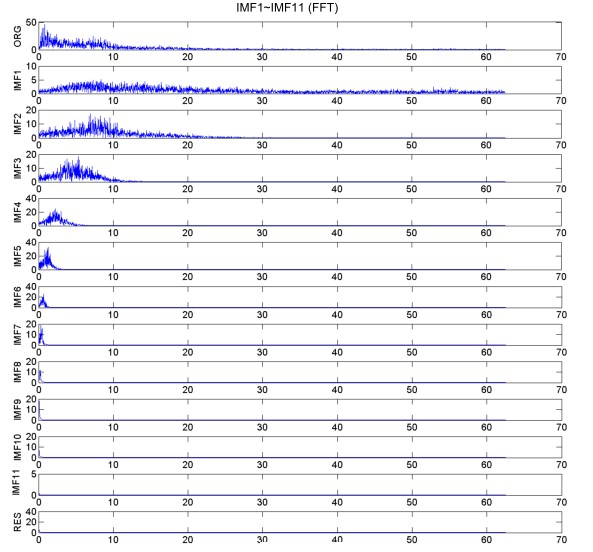
\includegraphics{IMF-Fre-FromPaper.jpg}
\caption{论文中的结果} \label{fig:IMF-Fre-FromPaper}
\end{figure}

\subsection{降噪 CutoffNoice.py}

在频域中,很容易得到噪声信号和有效信号。\colorbox{LetMeFlyGray}{CutoffNoice.py}将IMF中的噪声剔除。

\subsubsection{简介}

论文中已经给出了降噪的方式,因此这一步的主要任务就是将频率映射到给定范围内,并将不属于0.5HZ到32HZ的信号置零。

\begin{lstlisting}[language={python},
numbers=left,
numberstyle=\tiny\monaco,
basicstyle=\footnotesize\monaco]
from Visualize import showIMFs
from BaseClass import Data

def cutoffNoise(IMFs: Data) -> Data:
    originalMaxVal = []
    resizeRate = 35
    for th, IMF in enumerate(IMFs.data):
        maxVal = IMF.max()
        originalMaxVal.append(maxVal)
        IMFs.data[th] = IMF * resizeRate / maxVal
    IMFs.data[IMFs.data < 0.5] = 0
    IMFs.data[IMFs.data > 32] = 0
    showIMFs(IMFs, "Cut off noise")
    for th, IMF in enumerate(IMFs.data):
        IMFs.data[th] = IMF * originalMaxVal[th] / resizeRate
    return IMFs
\end{lstlisting}

\subsubsection{实现效果}

\begin{figure}[H]
\small
\centering
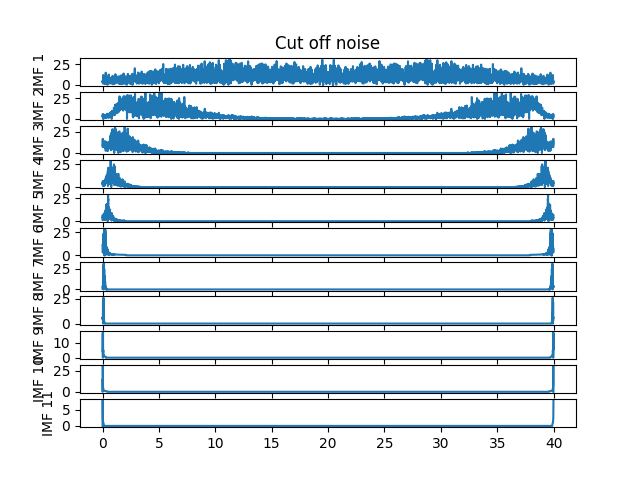
\includegraphics{cutoffnoise.png}
\caption{降噪} \label{fig:cutoffnoise}
\end{figure}

\subsection{将IMF转换回时域 IMF2TimeDomain.py}

\colorbox{LetMeFlyGray}{IMF2TimeDomain.py}将降噪后的IMF再次转换回时域。

\subsection{简介}

将IMF转换回时域主要使用快速傅里叶变换逆变换。这里同样使用了numpy中的ifft库。

可视化显示来自抽象出的显示函数。

\begin{lstlisting}[language={python},
numbers=left,
numberstyle=\tiny\monaco,
basicstyle=\footnotesize\monaco]
import numpy as np
from BaseClass import Data
from Visualize import showIMFs

def IMF2TimeDomain(IMFs: Data) -> Data:
    for i in range(len(IMFs.data)):
        IMFs.data[i] = np.fft.ifft(IMFs.data[i])
    
    showIMFs(IMFs, "Back to time domain")
    return IMFs

\end{lstlisting}

\subsubsection{实现效果}

\begin{figure}[H]
\small
\centering
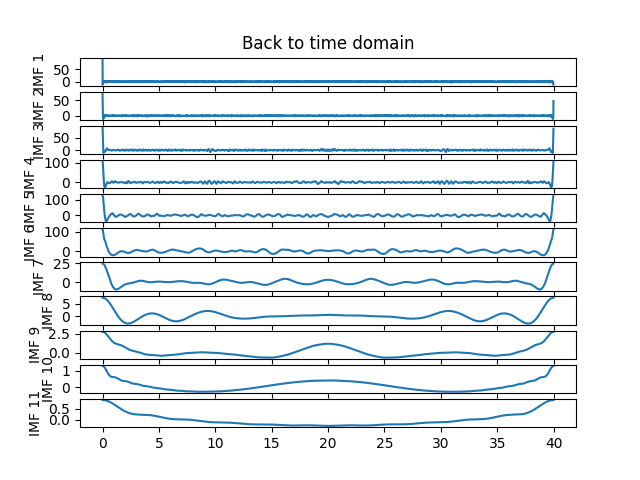
\includegraphics{backtotimedomain.png}
\caption{转换回频域} \label{fig:backtotimedomain}
\end{figure}

这里和论文中一样,出现了边缘效应

\begin{figure}[H]
\small
\centering
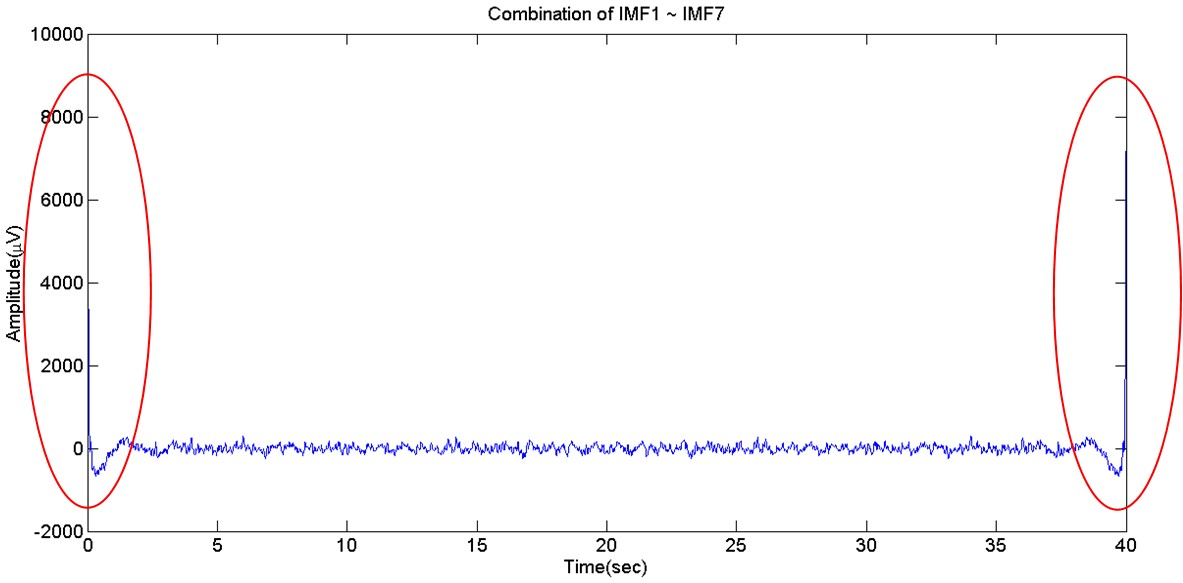
\includegraphics[width=\textwidth]{edge.jpg}
\caption{论文中的边缘效应} \label{fig:edge}
\end{figure}

\subsection{将IMF构建回EEG ConstructEEG.py}

\colorbox{LetMeFlyGray}{ConstructEEG.py}将IMF构建回EEG

\subsubsection{简介}

将IMF构建回EEG相比于其他步骤而言就显得更加容易,只需要将IMF叠加即可。

在叠加之前,先去除IFFT产生的边缘效应,之后将较小的IMF丢弃。

\begin{lstlisting}[language={python},
numbers=left,
numberstyle=\tiny\monaco,
basicstyle=\footnotesize\monaco]
from Visualize import showIMFs, showEEG
from BaseClass import Data

def ConstructEEG(IMFs: Data) -> Data:
    # 丢掉国小的IMF
    IMFs.setSubDataByPoints(200, 200)

    showIMFs(IMFs, "Remove edge effects data")

    # 丢弃过小的IMF
    IMFs.data = IMFs.data[:6]
    showIMFs(IMFs, "Desert small IMFs")

    EEG = Data(IMFs.data.sum(axis=0), IMFs.getStartTime(), IMFs.getFPS())
    showEEG(EEG, "Construct EEG")
    # EEG = EEG[1000:]
    # ax = plt.subplot()
    # ax.set_title('Construct EEG')
    # ax.plot(np.arange(0, end - start, 0.01), EEG)
    # plt.show()
    return EEG

\end{lstlisting}

\subsubsection{实现效果}

\begin{figure}[H]
\small
\centering
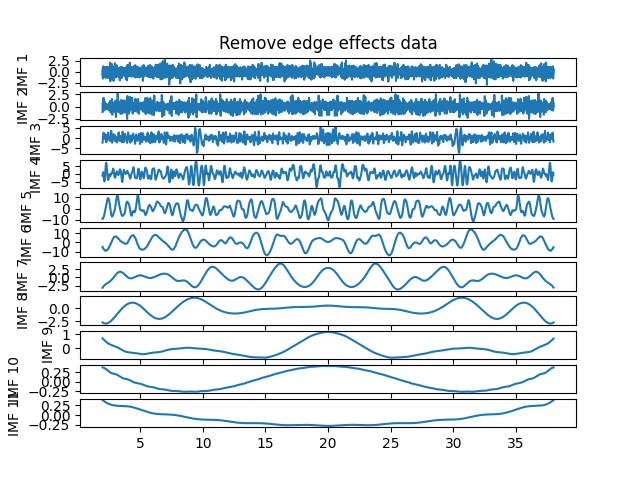
\includegraphics{remove-edge.png}
\caption{去除边缘} \label{fig:remove-edge}
\end{figure}

\begin{figure}[H]
\small
\centering
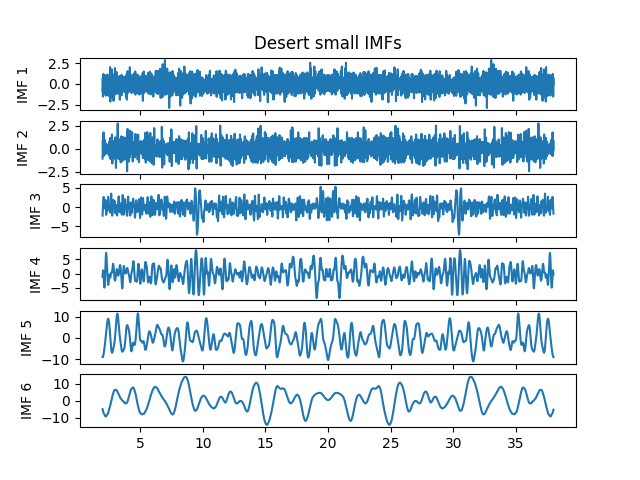
\includegraphics{desertSmallIMF.png}
\caption{丢弃较小的IMF} \label{fig:desertSmallIMF}
\end{figure}

\begin{figure}[H]
\small
\centering
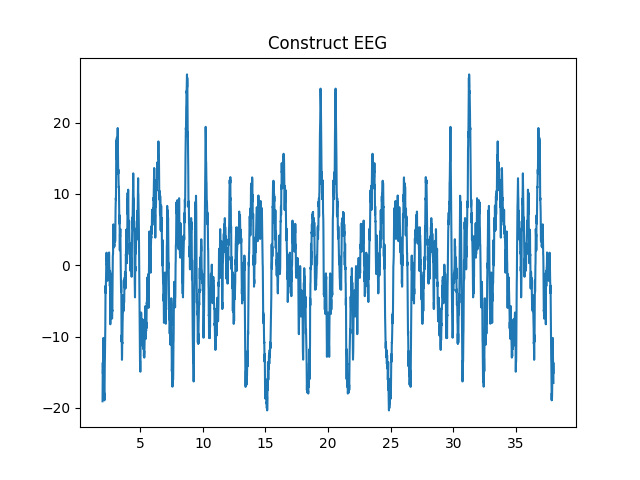
\includegraphics{newEEG.png}
\caption{合并成EEG} \label{fig:newEEG}
\end{figure}

\begin{figure}[H]
\small
\centering
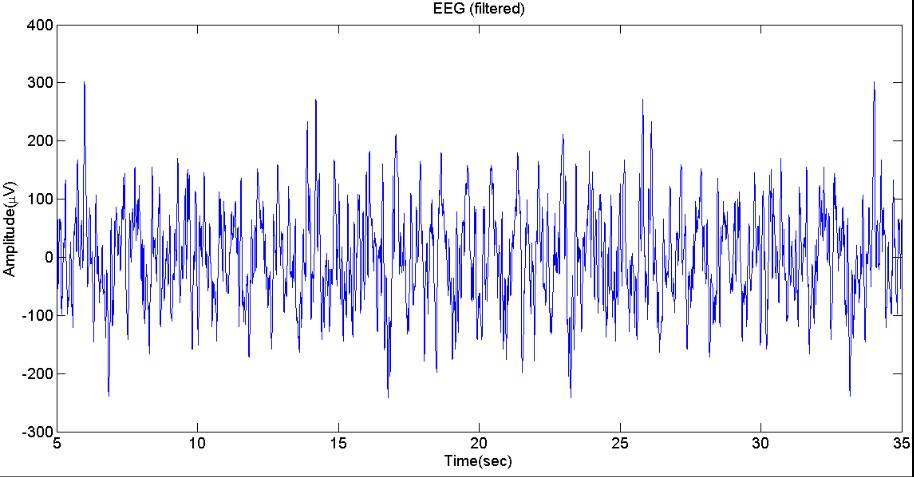
\includegraphics[width=\textwidth]{EEG-FromPaper.jpg}
\caption{论文中合并成的EEG} \label{fig:EEG-FromPaper}
\end{figure}

\subsection{希尔伯特-黄变换 HHT.py}

\colorbox{LetMeFlyGray}{HHT.py}通过HHT获得实时频率。

\subsubsection{简介}

希尔伯特-黄变换我也使用了scipy中的现成的库,学习自\url{https://blog.csdn.net/rouranling/article/details/123071180}

\begin{lstlisting}[language={python},
numbers=left,
numberstyle=\tiny\monaco,
basicstyle=\footnotesize\monaco]
from scipy.signal import hilbert
import numpy as np
from Visualize import showEEG
from BaseClass import Data

def HHT(EEG: Data) -> Data:
    analytic_signal = hilbert(EEG.data)
    amplitude_envelope = np.abs(analytic_signal)
    instantaneous_phase = np.unwrap(np.angle(analytic_signal))
    instantaneousFrequency = (np.diff(instantaneous_phase) / (2.0 * np.pi) * EEG.getFPS())
    # 上面instantaneousFrequency.shape = (3599,)
    instantaneousFrequency = np.append(instantaneousFrequency, 0)

    instantaneousFrequency = Data(instantaneousFrequency, EEG.getStartTime(), EEG.getFPS())
    showEEG(instantaneousFrequency, "HHT")

    return instantaneousFrequency
\end{lstlisting}

\subsubsection{实现效果}

\begin{figure}[H]
\small
\centering
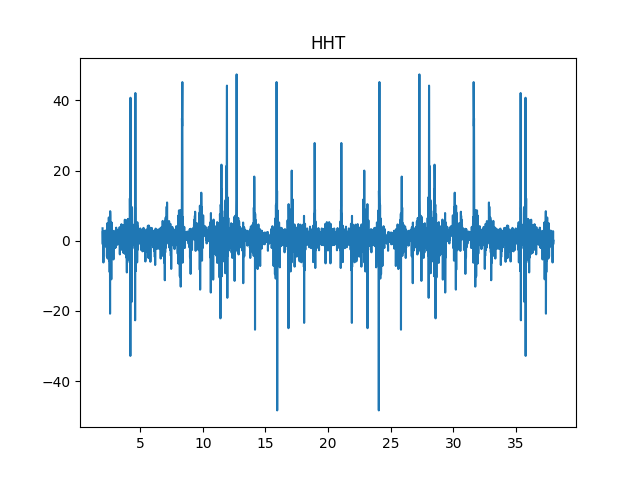
\includegraphics[width=\textwidth]{HHT.png}
\caption{希尔伯特黄变换} \label{fig:HHT}
\end{figure}

\subsection{显示实时三维图 ShowRealtime3D.py}

\subsubsection{简介}

\colorbox{LetMeFlyGray}{ShowRealtime3D.py}将通过HHT变换后的信号显示为实时三维图,并和论文中的结果做对比。

\begin{lstlisting}[language={python},
numbers=left,
numberstyle=\tiny\monaco,
basicstyle=\footnotesize\monaco]
from Visualize import show3d
import numpy as np
from BaseClass import Data

def showRealtime3D(EEG: Data, instantaneousFrequency: Data) -> None:
    show3d(instantaneousFrequency, EEG)
    show3d(instantaneousFrequency, EEG, ColorfulAndResize=True)
\end{lstlisting}

\subsubsection{实现效果}

\begin{figure}[H]
\small
\centering
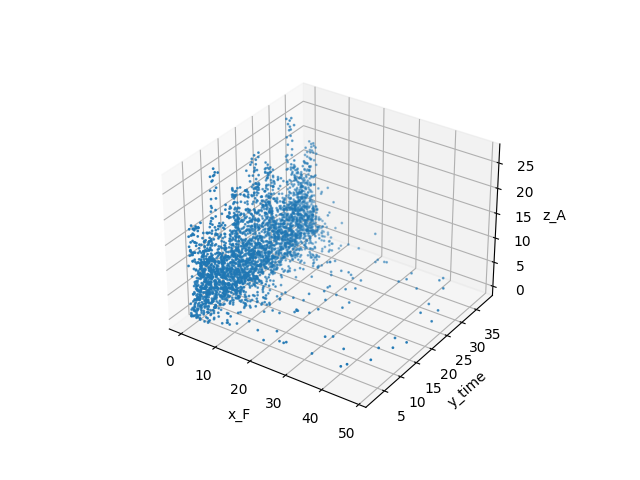
\includegraphics{3D.png}
\caption{3D散点图} \label{fig:3D}
\end{figure}

刚实现的效果猛的一看,还以为和论文中的不太一样。但是仔细分析后发现,不同之处主要来自两个方面

\begin{enumerate}
    \item 论文中相位纵坐标很高,因此论文中图像整体较扁
    \item 论文中的散点图颜色不同
\end{enumerate}

因此,我将图像压扁并对不同种类的波形加上不同的颜色,发现和论文中的实现效果很像!

\begin{figure}[H]
\small
\centering
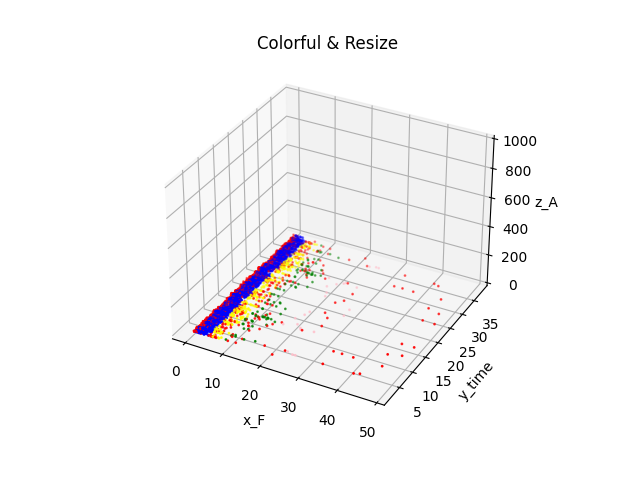
\includegraphics{3D-formatted.png}
\caption{格式化3D散点图} \label{fig:3D-formatted}
\end{figure}

\begin{figure}[H]
\small
\centering
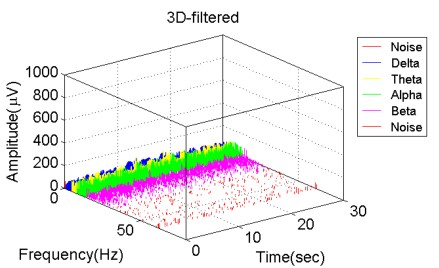
\includegraphics{3D-paper.jpg}
\caption{论文中的最终3D散点图} \label{fig:3D-paper}
\end{figure}

\subsection{基本功能类 BaseFunction.py}

\colorbox{LetMeFlyGray}{BaseFunction.py}实现了一些EEG信号处理领域所需的功能

\subsubsection{简介}

这里不得不提一句,本来专门抽象出这个\colorbox{LetMeFlyGray}{.py}文件是想着到后面可能会有很多地方再次用到这些较为基础的功能,但是到最后发现几乎只有\colorbox{LetMeFlyGray}{用到了这个文件里的函数}

此文件中实现了:

\begin{enumerate}
    \item ChangeToSameType:将两个数据转换为相同的numpy的类型
    \item formatTimeArray:规范化时间数组,使其不会在微小值上爆炸。返回的数组从0开始,最小增量为1。
    \item MyCubicSpline:三次样条曲线,原因是scipy.interpolate.interp1d不支持少于4个点的三次样条曲线
    \item peekDetection:极值检测
\end{enumerate}

\subsubsection{ChangeToSameType}

原理很简单,调用numpy中的find\_common\_type函数,然后把不是这个类型的数据强制转换为这个类型

\begin{lstlisting}[language={python},
numbers=left,
numberstyle=\tiny\monaco,
basicstyle=\footnotesize\monaco]
def ChangeToSameType(x: np.ndarray, y: np.ndarray):
    dtype = np.find_common_type([x.dtype, y.dtype], [])
    if x.dtype != dtype:
        x = x.astype(dtype)
    if y.dtype != dtype:
        y = y.astype(dtype)
    return x, y
\end{lstlisting}

\subsubsection{formatTimeArray}

规范化时间数组,使其不会在微小值上爆炸。返回的数组从0开始,最小增量为1。

\begin{lstlisting}[language={python},
numbers=left,
numberstyle=\tiny\monaco,
basicstyle=\footnotesize\monaco]
def formatTimeArray(t):
    d = np.diff(t)
    return (t - t[0]) / np.min(d)
\end{lstlisting}

\subsubsection{MyCubicSpline}

幸好之前数字图像处理课上学过三次样条插值曲线,但是还是参考了很多博客:\url{https://blog.csdn.net/bodybo/article/details/77335129}、\url{https://www.pythonheidong.com/blog/article/327241/58759b5470b375eb4f6d}

\begin{lstlisting}[language={python},
numbers=left,
numberstyle=\tiny\monaco,
basicstyle=\footnotesize\monaco]
def MyCubicSpline(x, y, T):
    
    x0, x1, x2 = x
    y0, y1, y2 = y

    x1x0, x2x1 = x1 - x0, x2 - x1
    y1y0, y2y1 = y1 - y0, y2 - y1
    _x1x0, _x2x1 = 1.0 / x1x0, 1.0 / x2x1

    m11, m12, m13 = 2 * _x1x0, _x1x0, 0
    m21, m22, m23 = _x1x0, 2.0 * (_x1x0 + _x2x1), _x2x1
    m31, m32, m33 = 0, _x2x1, 2.0 * _x2x1

    v1 = 3 * y1y0 * _x1x0 * _x1x0
    v3 = 3 * y2y1 * _x2x1 * _x2x1
    v2 = v1 + v3

    M = np.array([[m11, m12, m13], [m21, m22, m23], [m31, m32, m33]])
    v = np.array([v1, v2, v3]).T
    k = np.array(np.linalg.inv(M).dot(v))

    a1 = k[0] * x1x0 - y1y0
    b1 = -k[1] * x1x0 + y1y0
    a2 = k[1] * x2x1 - y2y1
    b2 = -k[2] * x2x1 + y2y1

    t = T[np.r_[T >= x0] & np.r_[T <= x2]]
    t1 = (T[np.r_[T >= x0] & np.r_[T < x1]] - x0) / x1x0
    t2 = (T[np.r_[T >= x1] & np.r_[T <= x2]] - x1) / x2x1
    t11, t22 = 1.0 - t1, 1.0 - t2

    q1 = t11 * y0 + t1 * y1 + t1 * t11 * (a1 * t11 + b1 * t1)
    q2 = t22 * y1 + t2 * y2 + t2 * t22 * (a2 * t22 + b2 * t2)
    q = np.append(q1, q2)

    return t, q
\end{lstlisting}

\subsubsection{peekDetection}

我不是很懂这样做的意义,但还是跟着参考资料这也做了

\begin{lstlisting}[language={python},
numbers=left,
numberstyle=\tiny\monaco,
basicstyle=\footnotesize\monaco]
def peekDetection(T: np.ndarray, S: np.ndarray):
    S1, S2 = S[:-1], S[1:]
    indexEr = np.nonzero(S1 * S2 < 0)[0]
    if np.any(S == 0):
        indexZero = np.nonzero(S == 0)[0]
        if np.any(np.diff(indexZero) == 1):
            zero = S == 0
            diff = np.diff(np.append(np.append(0, zero), 0))
            one = np.nonzero(diff == 1)[0]
            fuOne = np.nonzero(diff == -1)[0] - 1
            indexZero = np.round((one + fuOne) / 2.0)
        indexEr = np.sort(np.append(indexEr, indexZero))

    # 找到局部极值
    d = np.diff(S)
    d1, d2 = d[:-1], d[1:]
    indexMin = np.nonzero(np.r_[d1 * d2 < 0] & np.r_[d1 < 0])[0] + 1
    indexMax = np.nonzero(np.r_[d1 * d2 < 0] & np.r_[d1 > 0])[0] + 1

    # 如果有多个点具有相同的值
    if np.any(d == 0):
        imax, imin = [], []
        bad = d == 0
        dd = np.diff(np.append(np.append(0, bad), 0))
        debs = np.nonzero(dd == 1)[0]
        fins = np.nonzero(dd == -1)[0]
        if debs[0] == 1:
            if len(debs) > 1:
                debs, fins = debs[1:], fins[1:]
            else:
                debs, fins = [], []

        if len(debs) > 0:
            if fins[-1] == len(S) - 1:
                if len(debs) > 1:
                    debs, fins = debs[:-1], fins[:-1]
                else:
                    debs, fins = [], []

        lc = len(debs)
        if lc > 0:
            for k in range(lc):
                if d[debs[k] - 1] > 0:
                    if d[fins[k]] < 0:
                        imax.append(np.round((fins[k] + debs[k]) / 2.0))
                else:
                    if d[fins[k]] > 0:
                        imin.append(np.round((fins[k] + debs[k]) / 2.0))

        if len(imax) > 0:
            indexMax = indexMax.tolist()
            for x in imax:
                indexMax.append(int(x))
            indexMax.sort()

        if len(imin) > 0:
            indexMin = indexMin.tolist()
            for x in imin:
                indexMin.append(int(x))
            indexMin.sort()

    return T[indexMax], S[indexMax], T[indexMin], S[indexMin], indexEr  # 局部最大值的下标、局部最大值、局部最小值的坐标、局部最小值、index

\end{lstlisting}

\subsection{EEG信号的EMD分解 LetEMD.py}

\colorbox{LetMeFlyGray}{LetEMD.py}实现了EEG信号的EMD分解

\subsubsection{简介}

这个代码我写了200多行,参考了\url{https://github.com/laszukdawid/PyEMD}很多,但是都是手打的,调试了好久。同时也参考了\url{https://blog.csdn.net/The_Time_Runner/article/details/100882454}、\url{https://blog.csdn.net/weixin_39781323/article/details/115808594}很多地方并不是很懂。

主要包括:

\begin{enumerate}
    \item EMD主函数
    \item 提取最大和最小样条
    \item 镜像操作
    \item 三次样条曲线
    \item 是否停止分解
    \item 是否为IMF
\end{enumerate}

等功能。

\begin{lstlisting}[language={python},
numbers=left,
numberstyle=\tiny\monaco,
basicstyle=\footnotesize\monaco]
import numpy as np
from scipy.interpolate import interp1d
import BaseFunction


class EMD():
    def __init__(self):
        self.nbsym = 2
        self.dtype = np.float64
        self.IMFs = None
        self.residue = None

    def emd(self, S, T=None, max_imf=-1):
        T = np.arange(0, len(S), dtype=S.dtype)
        T = BaseFunction.formatTimeArray(T)
        S, T = BaseFunction.ChangeToSameType(S, T)
        oldIMF = np.nan
        IMFNum = 0
        EXTNum = -1
        self.dtype = S.dtype
        residue = S.astype(self.dtype)
        IMF = np.zeros(len(S), dtype=self.dtype)
        IMF2 = np.empty((IMFNum, len(S)))
        
        done = False
        while not done:
            residue[:] = S - np.sum(IMF2[:IMFNum], axis=0)
            IMF = residue.copy()
            mean = np.zeros(len(S), dtype=self.dtype)
            n = 0
            while True:
                n += 1
                if n >= 1000:  # 设置为最多执行1000次
                    print("数据过大或发生了死循环!")
                    break
                residueEXT = BaseFunction.peekDetection(T, IMF)
                maxLoc, minLoc, indexer = residueEXT[0], residueEXT[2], residueEXT[4]
                EXTNum = len(minLoc) + len(maxLoc)
                nzm = len(indexer)
                if EXTNum > 2:
                    envMax, envMin, eMax, eMin = self.extractMaxAndMinSpline(T, IMF)
                    mean[:] = 0.5 * (envMax + envMin)
                    oldIMF = IMF.copy()
                    IMF[:] = IMF - mean
                    # -------------
                    residueEXT = BaseFunction.peekDetection(T, IMF)
                    maxLoc, temp, minLoc, temp, indexer_ = residueEXT
                    EXTNum = len(maxLoc) + len(minLoc)
                    nzm = len(indexer_)
                    if oldIMF is np.nan:
                        continue
                    if self.ifIsIMF(IMF, oldIMF, eMax, eMin) and abs(EXTNum - nzm) < 2:
                        break
                else:
                    done = True
                    break
            IMF2 = np.vstack((IMF2, IMF.copy()))
            IMFNum += 1
            if self.timeToStop(S, IMF2) or IMFNum == max_imf:
                done = True
                break
        self.IMFs = IMF2.copy()
        self.residue = S - np.sum(self.IMFs, axis=0)
        return self.IMFs, self.residue

    def extractMaxAndMinSpline(self, T: np.ndarray, S: np.ndarray):
        extremaLoc = BaseFunction.peekDetection(T, S)
        maxLoc, maxVal = extremaLoc[0], extremaLoc[1]
        minLoc, minVal = extremaLoc[2], extremaLoc[3]
        if len(maxLoc) + len(minLoc) < 3:
            return [-1] * 4
        maxExtrema, minExtrema = self.preparePoints(T, S, maxLoc, maxVal, minLoc, minVal)
        temp, maxSpline = self.cubicSpline(T, maxExtrema)
        temp, minSpline = self.cubicSpline(T, minExtrema)
        return maxSpline, minSpline, maxExtrema, minExtrema

    """
    镜像操作
    """
    def preparePoints(self, T, S, maxLoc, maxVal, minLoc, minVal):
        # 至少需要两个极值
        maxExtrema = np.zeros((2, len(maxLoc)), dtype=self.dtype)
        minExtrema = np.zeros((2, len(minLoc)), dtype=self.dtype)
        maxExtrema[0], minExtrema[0] = maxLoc, minLoc
        maxExtrema[1], minExtrema[1] = maxVal, minVal
        nbsym = self.nbsym
        minEnd, maxEnd = len(minLoc), len(maxLoc)
        # 左边界
        locD = maxLoc[0] - minLoc[0]
        ifLeftExtremaIsMax = locD < 0  # 如果locD < 0,那么leftExtremaMaxType就为True,就说明为左极值最大值;否则为最小值

        # 左极值为最大值
        if ifLeftExtremaIsMax:
            if (S[0] > minVal[0]) and (np.abs(locD) > (maxLoc[0] - T[0])):
                # 第一个极值
                expandLeftMaxPos = 2 * maxLoc[0] - maxLoc[1 : nbsym + 1]
                expandLeftMinPos = 2 * maxLoc[0] - minLoc[0:nbsym]
                expandLeftMaxVal = maxVal[1 : nbsym + 1]
                expandLeftMinVal = minVal[0:nbsym]
            else:
                # 起始位置
                expandLeftMaxPos = 2 * T[0] - maxLoc[0:nbsym]
                expandLeftMinPos = 2 * T[0] - np.append(T[0], minLoc[0 : nbsym - 1])
                expandLeftMaxVal = maxVal[0:nbsym]
                expandLeftMinVal = np.append(S[0], minVal[0 : nbsym - 1])
        # 左极值为最小值
        else:
            if (S[0] < maxVal[0]) and (np.abs(locD) > (minLoc[0] - T[0])):
                # 第一个极值
                expandLeftMaxPos = 2 * minLoc[0] - maxLoc[0:nbsym]
                expandLeftMinPos = 2 * minLoc[0] - minLoc[1 : nbsym + 1]
                expandLeftMaxVal = maxVal[0:nbsym]
                expandLeftMinVal = minVal[1 : nbsym + 1]
            else:
                # 起始位置
                expandLeftMaxPos = 2 * T[0] - np.append(T[0], maxLoc[0 : nbsym - 1])
                expandLeftMinPos = 2 * T[0] - minLoc[0:nbsym]
                expandLeftMaxVal = np.append(S[0], maxVal[0 : nbsym - 1])
                expandLeftMinVal = minVal[0:nbsym]

        if not expandLeftMinPos.shape:
            expandLeftMinPos, expandLeftMinVal = minLoc, minVal
        if not expandLeftMaxPos.shape:
            expandLeftMaxPos, expandLeftMaxVal = maxLoc, maxVal
        expandLeftMin = np.vstack((expandLeftMinPos[::-1], expandLeftMinVal[::-1]))
        expandLeftMax = np.vstack((expandLeftMaxPos[::-1], expandLeftMaxVal[::-1]))

        # 右边界
        locD = maxLoc[-1] - minLoc[-1]
        rightExtremaMaxYype = locD > 0
        # 右极值是最大值
        if not rightExtremaMaxYype:
            if (S[-1] < maxVal[-1]) and (np.abs(locD) > (T[-1] - minLoc[-1])):
                # 最后一个极值
                maxIndex = max(0, maxEnd - nbsym)
                minIndex = max(0, minEnd - nbsym - 1)
                expandRightMaxLoc = 2 * minLoc[-1] - maxLoc[maxIndex:]
                expandRightMinPos = 2 * minLoc[-1] - minLoc[minIndex:-1]
                expandRightMaxVal = maxVal[maxIndex:]
                expandRightMinVal = minVal[minIndex:-1]
            else:
                # 终止位置
                maxIndex = max(0, maxEnd - nbsym + 1)
                minIndex = max(0, minEnd - nbsym)
                expandRightMaxLoc = 2 * T[-1] - np.append(maxLoc[maxIndex:], T[-1])
                expandRightMinPos = 2 * T[-1] - minLoc[minIndex:]
                expandRightMaxVal = np.append(maxVal[maxIndex:], S[-1])
                expandRightMinVal = minVal[minIndex:]
        # 右极值是最小值
        else:
            if (S[-1] > minVal[-1]) and len(maxLoc) > 1 and (np.abs(locD) > (T[-1] - maxLoc[-1])):
                # 最后一个极值
                maxIndex = max(0, maxEnd - nbsym - 1)
                minIndex = max(0, minEnd - nbsym)
                expandRightMaxLoc = 2 * maxLoc[-1] - maxLoc[maxIndex:-1]
                expandRightMinPos = 2 * maxLoc[-1] - minLoc[minIndex:]
                expandRightMaxVal = maxVal[maxIndex:-1]
                expandRightMinVal = minVal[minIndex:]
            else:
                # 终止位置
                maxIndex = max(0, maxEnd - nbsym)
                minIndex = max(0, minEnd - nbsym + 1)
                expandRightMaxLoc = 2 * T[-1] - maxLoc[maxIndex:]
                expandRightMinPos = 2 * T[-1] - np.append(minLoc[minIndex:], T[-1])
                expandRightMaxVal = maxVal[maxIndex:]
                expandRightMinVal = np.append(minVal[minIndex:], S[-1])

        if not expandRightMinPos.shape:
            expandRightMinPos, expandRightMinVal = minLoc, minVal
        if not expandRightMaxLoc.shape:
            expandRightMaxLoc, expandRightMaxVal = maxLoc, maxVal

        enpandRightMin = np.vstack((expandRightMinPos[::-1], expandRightMinVal[::-1]))
        expandRightMax = np.vstack((expandRightMaxLoc[::-1], expandRightMaxVal[::-1]))
        maxExtrema = np.hstack((expandLeftMax, maxExtrema, expandRightMax))
        minExtrema = np.hstack((expandLeftMin, minExtrema, enpandRightMin))
        return maxExtrema, minExtrema

    """
    三次样条
    """
    def cubicSpline(self, T: np.ndarray, extrema: np.ndarray):
        t = T[np.r_[T >= extrema[0, 0]] & np.r_[T <= extrema[0, -1]]]
        if extrema.shape[1] > 3:  # 大于三个点,使用内置库
            return t, interp1d(extrema[0], extrema[1], kind="cubic")(t)
        else:  # 否则还得手动实现一波
            return BaseFunction.MyCubicSpline(extrema[0], extrema[1], t)

    """
    是否停止分解
    对于剩下的数据,最大值和最小值之差小于0.001 或 绝对值之和小于0.005时,停止分解
    """
    def timeToStop(self, S: np.ndarray, IMF: np.ndarray) -> bool:
        remain = S - np.sum(IMF, axis=0)
        if np.max(remain) - np.min(remain) < 0.001:  # 这里设置为0.001 #--------------------
            return True
        if np.sum(np.abs(remain)) < 0.005:  # 这里设置为0.005 #--------------------
            return True
        return False

    """
    如果连续筛选不影响信号,则信号为IMF
    """
    def ifIsIMF(self, newIMF: np.ndarray, oldIMF: np.ndarray, eMax: np.ndarray, eMin: np.ndarray) -> bool:
        if np.any(eMax[1] < 0) or np.any(eMin[1] > 0):
            return False
        if np.sum(newIMF ** 2) < 1e-10:
            return False

        IMFDiff = newIMF - oldIMF
        PingFang = np.sum(IMFDiff ** 2)
        svar = PingFang / (max(oldIMF) - min(oldIMF))
        if svar < 0.001:  # svar_thr,定义为0.001
            return True

        # 标准差检验
        std = np.sum((IMFDiff / newIMF) ** 2)
        if std < 0.2:  # std_thr,定义为0.2
            return True
        energyRatio = PingFang / np.sum(oldIMF * oldIMF)
        if energyRatio < 0.2:  # energy_ratio_thr,定义为0.2
            return True
        return False
\end{lstlisting}


\section{未来展望}

\begin{enumerate}
\item 当前程序不支持命令行传参,也就是说默认采样频率是100,并且只能读取名为“case7.txt”的数据文件。不过这不是大问题。
\item 在去除“很小”的IMF时,论文中并未提出一种有效的由程序自动识别“什么是很小的IMF”的方法。未来可以在程序中添加这个功能,比如“最大值小于第一个IMF的1\%就视为小IMF”、“极差不超过多少就视为小IMF”等。
\item 我所实现的EMD分解不支持参数设置,如:分解为多少IMF、分解的终止条件等。
\item IFFT带来的边缘效应会使IMF两端的振幅特别地高。当前(论文中也类似)采用的办法是去除前200个采样点和后200个采样点。未来可以研究并使用一种更为“智能”的方法,让程序计算出前后应该分别去除多少个采样点以避免边缘效应。
\end{enumerate}








%===参考文献===
%\addcontentsline{toc}{section}{参考文献}
%\bibliographystyle{abbrv}     %论文引用格式
%\bibliography{E:/studio/wrtex/wrtkit/referbib/wholebiblio}
                         
\begin{thebibliography}{99}
\bibitem{A19}{\em Mu-Tzu Shih, Faiyaz Doctor, Shou-Zen Fan, Kuo-Kuang Jen and Jiann-Shing Shieh.  \href{https://www.mdpi.com/1099-4300/17/3/928}{\color{red}Instantaneous 3D EEG Signal Analysis Based on Empirical Mode Decomposition and the Hilbert–Huang Transform Applied to Depth of Anaesthesia}}, 2022.
\bibitem{A19}{\em \color{red}爱码网:matplotlib消除QT警告}. \href{https://www.likecs.com/ask-924744.html}{https://www.likecs.com/ask-924744.html}, 2022.
\bibitem{A19}{\em \color{red}CSDN:matplotlib显示三维散点图}. \href{https://blog.csdn.net/weixin\_46287157/article/details/124784731}{https://blog.csdn.net/weixin\_46287157/article/details/124784731}, 2022.
\bibitem{A19}{\em \color{red}脚本之家:不同频率的数据显示不同的颜色}. \href{https://www.jb51.net/article/258747.htm}{https://www.jb51.net/article/258747.htm}, 2022.
\bibitem{A19}{\em \color{red}figshare:深度麻醉数据集下载}. \href{https://figshare.com/articles/dataset/EEG\_and\_BIS\_raw\_data/5589841/1}{https://figshare.com/articles/dataset/EEG\_and\_BIS\_raw\_data/5589841/1}, 2022.
\bibitem{A19}{\em \color{red}CSDN: Matlab保存数据到文件}. \href{https://blog.csdn.net/whb12345678feng/article/details/103108114}{https://blog.csdn.net/whb12345678feng/article/details/103108114}, 2022.
\bibitem{A19}{\em \color{red}CSDN: Hilbert变换提取信号特征}. \href{https://blog.csdn.net/rouranling/article/details/123071180}{https://blog.csdn.net/rouranling/article/details/123071180}, 2022.
\bibitem{A19}{\em \color{red}CSDN: Cubic spline(三次样条插值)}. \href{https://blog.csdn.net/bodybo/article/details/77335129}{https://blog.csdn.net/bodybo/article/details/77335129}, 2022.
\bibitem{A19}{\em \color{red}Python黑洞网: 三次样条曲线}. \href{https://www.pythonheidong.com/blog/article/327241/58759b5470b375eb4f6d/}{https://www.pythonheidong.com/blog/article/327241/58759b5470b375eb4f6d/}, 2022.
\bibitem{A19}{\em \color{red}Github: PyEMD}. \href{https://github.com/laszukdawid/PyEMD}{https://github.com/laszukdawid/PyEMD}, 2022.
\bibitem{A19}{\em \color{red}CSDN: scipy.interpolate.interp1d()函数详解}. \href{https://blog.csdn.net/The\_Time\_Runner/article/details/100882454}{https://blog.csdn.net/The\_Time\_Runner/article/details/100882454}, 2022.
\bibitem{A19}{\em \color{red}CSDN: 如何检测一个信号的变换趋势是上升还是下降}. \href{https://blog.csdn.net/weixin\_39781323/article/details/115808594}{https://blog.csdn.net/weixin\_39781323/article/details/115808594}, 2022.

\end{thebibliography}
\end{document}
%===结束===



History:
2022-8-20: 依据程勇老师的Note.tex创建;



